% Figure 2 — ABM Forward Simulation Pipeline
% Sister figure to Figure 1 (ML Training Pipeline). Same 4-row Wang-style
% stacked layout. Receives "trained Θ" from Figure 1 as input.
%
% Row 1: Frozen Θ + Counterfactual intervention setup
% Row 2: Re-encoder forward + Agent dispatch (heterogeneity!)
% Row 3: BPR closure + MSA fixed-point iteration
% Row 4: Outputs · counterfactual welfare assessment
%
% Compile:  pdflatex figure2_abm_pipeline.tex

\documentclass[border=8pt]{standalone}

\usepackage[T1]{fontenc}
\usepackage{lmodern}
\usepackage{amsmath, amssymb}
\usepackage{tikz}
\usepackage{xcolor}
\usepackage{graphicx}

\usetikzlibrary{
  positioning, arrows.meta, shapes.geometric, calc, fit, backgrounds,
  matrix, decorations.pathmorphing,
}

% ─── Stage colour palette (different from Fig 1 to distinguish two figures) ──
\definecolor{stageABg}    {HTML}{F1F5F9}    % light slate (setup)
\definecolor{stageABanner}{HTML}{475569}
\definecolor{stageBBg}    {HTML}{FCE4C7}    % light orange (ABM core)
\definecolor{stageBBanner}{HTML}{C2410C}
\definecolor{stageCBg}    {HTML}{F5E6D8}    % light brown (BPR)
\definecolor{stageCBanner}{HTML}{92400E}
\definecolor{stageDBg}    {HTML}{D6EBE8}    % light teal (outputs)
\definecolor{stageDBanner}{HTML}{0F766E}

\definecolor{cFlow}       {HTML}{E07A5F}
\definecolor{cBPR}        {HTML}{F59E0B}
\definecolor{cText}       {HTML}{1F2937}
\definecolor{cMuted}      {HTML}{6B7280}
\definecolor{cBorder}     {HTML}{CBD5E1}
\definecolor{cIO}         {HTML}{0F766E}

% Parameter category colours (consistent with Figure 1 trained Θ)
\definecolor{cParEnc}   {HTML}{475569}
\definecolor{cParBeta}  {HTML}{C44E52}
\definecolor{cParGamma} {HTML}{F59E0B}
\definecolor{cParDelta} {HTML}{0E7490}
\definecolor{cParKappa} {HTML}{8172B2}

% Agent type colours (consistent with agent_heterogeneity.png)
\definecolor{cAgentWalk}   {HTML}{10B981}
\definecolor{cAgentTransit}{HTML}{F59E0B}
\definecolor{cAgentCar}    {HTML}{3B82F6}

\begin{document}

\begin{tikzpicture}[
  font=\sffamily\small,
  thick,
  >={Stealth[length=4.5pt, width=4pt]},
  every node/.style={align=center, text=cText},
  %
  rowframe/.style={
    draw=none, fill=#1, rounded corners=6pt,
    inner xsep=8pt, inner ysep=10pt,
  },
  rowbanner/.style={
    fill=#1, text=white, font=\sffamily\bfseries\small,
    rounded corners=4pt, inner sep=6pt,
  },
  modA/.style={
    draw=stageABanner, fill=white, line width=0.7pt,
    rounded corners=3pt, inner sep=5pt,
  },
  modB/.style={
    draw=stageBBanner, fill=white, line width=0.7pt,
    rounded corners=3pt, inner sep=5pt,
  },
  modC/.style={
    draw=stageCBanner, fill=white, line width=0.7pt,
    rounded corners=3pt, inner sep=5pt,
  },
  modD/.style={
    draw=stageDBanner, fill=white, line width=0.7pt,
    rounded corners=3pt, inner sep=5pt,
  },
  arrFwd/.style={->, line width=1.6pt, draw=cFlow},
  arrInner/.style={->, line width=0.8pt, draw=cText!70},
  arrBPR/.style={->, line width=1.0pt, draw=cBPR, dashed},
  arrlbl/.style={font=\sffamily\scriptsize\itshape, text=cMuted, fill=white,
                 inner sep=1pt, midway},
  cellgrid/.style={draw=cMuted!50, fill=#1, line width=0.3pt, rectangle},
]

% ════════════════════════════════════════════════════════════════════════
%  ROW 1 · FROZEN Θ + COUNTERFACTUAL INTERVENTION
% ════════════════════════════════════════════════════════════════════════

\begin{scope}[local bounding box=row1]

  % ── Panel A1: Frozen Θ card (mini version of Figure 1's bridge) ──
  \node[modA, anchor=north west] (theta) at (0, 0)
    {\begin{minipage}{106mm}
      \centering\textbf{\textcolor{stageABanner}{\textcircled{\scriptsize 1} Trained $\Theta\bigstar$ frozen (received from Figure~1)}}\\[2pt]
      \scriptsize\textcolor{cIO}{IN: from Fig.~1}\;\;\textcolor{cIO}{OUT: 5 frozen parameter types}\\[3pt]
      \begin{tikzpicture}[baseline=0]
        % 5 mini parameter pills
        \node[draw=cParEnc, fill=cParEnc!10, rounded corners=2pt, line width=0.5pt,
               minimum width=18mm, minimum height=10mm,
               font=\sffamily\tiny, text=cParEnc]
              (penc) at (0, 0) {$\Theta_{\text{enc}}$\\\tiny 33{,}026};
        \node[draw=cParBeta, fill=cParBeta!10, rounded corners=2pt, line width=0.5pt,
               minimum width=18mm, minimum height=10mm,
               font=\sffamily\tiny, text=cParBeta,
               anchor=north west] (pbeta) at (20mm, 1.5mm)
             {$\beta_{t,m}$\\\tiny 72};
        \node[draw=cParGamma, fill=cParGamma!10, rounded corners=2pt, line width=0.5pt,
               minimum width=18mm, minimum height=10mm,
               font=\sffamily\tiny, text=cParGamma,
               anchor=north west] (pgamma) at (40mm, 1.5mm)
             {$\gamma$\\\tiny 1};
        \node[draw=cParDelta, fill=cParDelta!10, rounded corners=2pt, line width=0.5pt,
               minimum width=18mm, minimum height=10mm,
               font=\sffamily\tiny, text=cParDelta,
               anchor=north west] (pdelta) at (60mm, 1.5mm)
             {$\delta_k$\\\tiny 2};
        \node[draw=cParKappa, fill=cParKappa!10, rounded corners=2pt, line width=0.5pt,
               minimum width=18mm, minimum height=10mm,
               font=\sffamily\tiny, text=cParKappa,
               anchor=north west] (pkappa) at (80mm, 1.5mm)
             {$\kappa_k$\\\tiny 2};
        \node[font=\sffamily\tiny, text=cMuted, anchor=west] at (0, -8mm)
            {Total \textbf{33{,}103} params · \textbf{77 interpretable behavioural primitives} · NO re-fit at deployment};
      \end{tikzpicture}
    \end{minipage}};

  % ── Panel A2: Counterfactual Sc.A spatial intervention ──
  \node[modA, anchor=north west] (sca) at (114mm, 0)
    {\begin{minipage}{82mm}
      \centering\textbf{\textcolor{stageABanner}{\textcircled{\scriptsize 2a} Sc.\,A · do$(X^{\text{static}})$ — spatial}}\\[2pt]
      \scriptsize OOC cluster $+$65,000 jobs (9 grids around grid 908)\\[3pt]
      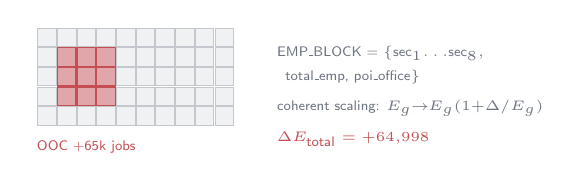
\begin{tikzpicture}[baseline=0]
        % London grid sketch with OOC 9-grid cluster highlighted
        \foreach \x in {0,...,9}{
          \foreach \y in {0,...,4}{
            \node[draw=cMuted!40, fill=cMuted!10, minimum size=2mm, line width=0.2pt]
                  at (\x*2.5mm, -\y*2.5mm) {};
          }
        }
        % OOC cluster (3x3 grid centred on x=2, y=2)
        \foreach \x in {1,2,3}{
          \foreach \y in {1,2,3}{
            \node[draw=cParBeta, fill=cParBeta!50, minimum size=2mm, line width=0.4pt]
                  at (\x*2.5mm, -\y*2.5mm) {};
          }
        }
        \node[font=\sffamily\tiny, text=cParBeta] at (5mm, -14mm) {OOC +65k jobs};
        % arrow + employment delta indicator
        \node[font=\sffamily\tiny, text=cMuted, anchor=west] at (28mm, -2mm)
              {EMP\_BLOCK = $\{\text{sec}_1{\dots}\text{sec}_8,$};
        \node[font=\sffamily\tiny, text=cMuted, anchor=west] at (28mm, -5mm)
              {\;\;total\_emp, poi\_office$\}$};
        \node[font=\sffamily\tiny, text=cMuted, anchor=west] at (28mm, -9mm)
              {coherent scaling: $E_g \!\!\to\!\! E_g (1{+}\Delta/E_g)$};
        \node[font=\sffamily\tiny, text=cParBeta, anchor=west] at (28mm, -13mm)
              {$\Delta E_{\text{total}} = +64{,}998$};
      \end{tikzpicture}
    \end{minipage}};

  % ── Panel A3: Counterfactual Sc.B temporal intervention ──
  \node[modA, anchor=north west] (scb) at (204mm, 0)
    {\begin{minipage}{96mm}
      \centering\textbf{\textcolor{stageABanner}{\textcircled{\scriptsize 2b} Sc.\,B · do$(X^{\text{dyn}})$ — temporal}}\\[2pt]
      \scriptsize Flexible work: peak $\!\times\!0.5$, shoulder $\!\times\!1.5$ (mass-conserved)\\[3pt]
      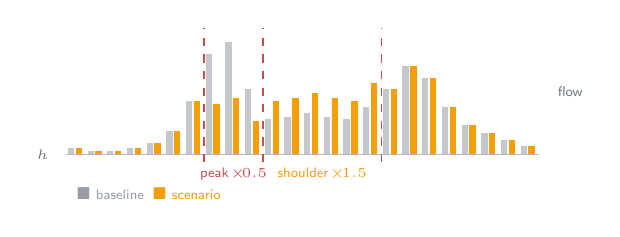
\begin{tikzpicture}[baseline=0]
        % 24-hour profile: baseline (gray) vs intervened (orange)
        % baseline curve mock (high at 7-9 and 17-19)
        \foreach \h/\base/\scen in
          {0/0.05/0.05, 1/0.03/0.03, 2/0.03/0.03, 3/0.05/0.05, 4/0.10/0.10,
           5/0.20/0.20, 6/0.45/0.45, 7/0.85/0.43, 8/0.95/0.48, 9/0.55/0.28,
           10/0.30/0.45, 11/0.32/0.48, 12/0.35/0.52, 13/0.32/0.48, 14/0.30/0.45,
           15/0.40/0.60, 16/0.55/0.55, 17/0.75/0.75, 18/0.65/0.65, 19/0.40/0.40,
           20/0.25/0.25, 21/0.18/0.18, 22/0.12/0.12, 23/0.07/0.07}{
          % baseline gray bar
          \fill[cMuted!40] (\h*2.5mm + 0.2mm, 0) rectangle (\h*2.5mm + 1.0mm, \base*15mm);
          % scenario orange bar
          \fill[cParGamma] (\h*2.5mm + 1.2mm, 0) rectangle (\h*2.5mm + 2.0mm, \scen*15mm);
        }
        \draw[cMuted!50, line width=0.3pt] (0, 0) -- (60mm, 0);
        % peak/shoulder bands
        \draw[cParBeta, line width=0.5pt, dashed]
            (7*2.5mm, -1mm) -- (7*2.5mm, 16mm)
            (10*2.5mm, -1mm) -- (10*2.5mm, 16mm)
            (16*2.5mm, -1mm) -- (16*2.5mm, 16mm);
        \node[font=\sffamily\tiny, text=cParBeta] at (8.5*2.5mm, -2.5mm) {peak $\!\times\!0.5$};
        \node[font=\sffamily\tiny, text=cParGamma] at (13*2.5mm, -2.5mm) {shoulder $\!\times\!1.5$};
        \node[font=\sffamily\tiny, text=cMuted] at (-3mm, 0) {$h$};
        \node[font=\sffamily\tiny, text=cMuted] at (24*2.5mm + 4mm, 8mm) {flow};
        % Legend
        \node[font=\sffamily\tiny, text=cMuted, anchor=west] at (0, -5mm)
            {\textcolor{cMuted!70}{$\blacksquare$ baseline}\;\;\textcolor{cParGamma}{$\blacksquare$ scenario}};
      \end{tikzpicture}
    \end{minipage}};

\end{scope}

\begin{pgfonlayer}{background}
  \node[rowframe=stageABg, fit=(row1)] (frameRow1) {};
\end{pgfonlayer}
\node[rowbanner=stageABanner, anchor=north west]
  at ($(frameRow1.north west)+(8pt, 0pt)$)
  {\textsc{Stage A · Frozen $\Theta$ + Counterfactual intervention}\;\,\textmd{\itshape — set up the deployment scenario}};

% ════════════════════════════════════════════════════════════════════════
%  ROW 2 · RE-ENCODER + AGENT DISPATCH (the heterogeneity core)
% ════════════════════════════════════════════════════════════════════════

\begin{scope}[local bounding box=row2, shift={(0, -68mm)}]

  % ── Panel B1: Re-encoder (frozen) ──
  \node[modB, anchor=north west] (renc) at (0, 0)
    {\begin{minipage}{72mm}
      \centering\textbf{\textcolor{stageBBanner}{\textcircled{\scriptsize 3} Re-encode under intervention}}\\[2pt]
      \scriptsize\textcolor{cIO}{IN: $X^{\text{perturbed}}, \Theta_{\text{enc}}\!\bigstar$}\;\;\textcolor{cIO}{OUT: $V^{\,\prime}_{j,t}$}\\[3pt]
      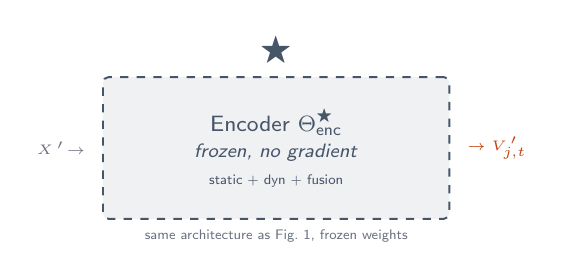
\begin{tikzpicture}[baseline=0]
        % Encoder box (frozen indicator)
        \node[draw=cParEnc, fill=cParEnc!8, rounded corners=2pt, dashed,
               line width=0.7pt, minimum width=44mm, minimum height=18mm,
               font=\sffamily\footnotesize, text=cParEnc, align=center] (enc) at (0, 0)
             {Encoder $\Theta_{\text{enc}}^{\bigstar}$\\\scriptsize\textit{frozen, no gradient}\\\tiny static + dyn + fusion};
        % Input/output arrows
        \node[font=\sffamily\tiny, text=cMuted, anchor=east] at (-23mm, 0) {$X^{\,\prime}\!\to$};
        \node[font=\sffamily\tiny, text=stageBBanner, anchor=west] at (23mm, 0) {$\to V^{\,\prime}_{j,t}$};
        % Lock symbol
        \node[font=\sffamily\large, text=cParEnc, anchor=south]
              at (enc.north) {$\bigstar$};
        \node[font=\sffamily\tiny, text=cMuted, anchor=north]
              at (enc.south) {same architecture as Fig.~1, frozen weights};
      \end{tikzpicture}
    \end{minipage}};

  % ── Panel B2: Agent population sampling ──
  \node[modB, anchor=north west] (asample) at (80mm, 0)
    {\begin{minipage}{60mm}
      \centering\textbf{\textcolor{stageBBanner}{\textcircled{\scriptsize 4} Agent population sampling}}\\[2pt]
      \scriptsize\textcolor{cIO}{IN: $\pi_m(i), \pi_k(i)$}\;\;\textcolor{cIO}{OUT: $N$ agents}\\[3pt]
      \begin{tikzpicture}[baseline=0]
        % π_m × π_k joint distribution
        \node[font=\sffamily\tiny, text=cText] at (16mm, 12mm) {joint distribution $\pi_m(i)\!\times\!\pi_k(i)$};
        % small 3x3 mode×tier matrix
        \foreach \r/\m in {0/car, 1/tr, 2/wk}
          \foreach \c/\k in {0/lo, 1/mi, 2/hi}{
            \pgfmathsetmacro{\val}{0.2 + 0.15*(\r+\c)}
            \node[cellgrid=stageBBanner, minimum size=3mm, opacity=\val]
                  at (8mm + \c*3mm, 7mm - \r*3mm) {};
          }
        \node[font=\sffamily\tiny, text=cMuted] at (12mm, -2mm) {$3\!\times\!3 = 9$ types};
        % arrow to agents
        \draw[->, line width=0.8pt, draw=stageBBanner] (22mm, 4mm) -- (28mm, 4mm);
        % stick-figure agents
        \foreach \i/\xoff/\col in
          {1/30/cAgentWalk, 2/35/cAgentTransit, 3/40/cAgentCar,
           4/45/cAgentWalk, 5/50/cAgentTransit, 6/55/cAgentCar}{
          \node[circle, fill=\col, minimum size=1.5mm, inner sep=0pt]
                at (\xoff mm, 7mm) {};
          \draw[\col, line width=0.6pt] (\xoff mm, 6mm) -- (\xoff mm, 3mm);
          \draw[\col, line width=0.5pt] (\xoff mm - 1mm, 4.5mm) -- (\xoff mm + 1mm, 4.5mm);
          \draw[\col, line width=0.5pt] (\xoff mm, 3mm) -- (\xoff mm - 1mm, 1mm);
          \draw[\col, line width=0.5pt] (\xoff mm, 3mm) -- (\xoff mm + 1mm, 1mm);
        }
        \node[font=\sffamily\tiny, text=cMuted] at (42mm, -2mm) {$N$ agents drawn};
      \end{tikzpicture}
    \end{minipage}};

  % ── Panel B3: Agent heterogeneity — KEY VISUALIZATION ──
  \node[modB, anchor=north west] (ahet) at (148mm, 0)
    {\begin{minipage}{152mm}
      \centering\textbf{\textcolor{stageBBanner}{\textcircled{\scriptsize 5} Per-agent personalised parameters $\to$ Gumbel-max choice}}\\[2pt]
      \scriptsize\textcolor{cIO}{IN: $V^{\,\prime}_{j,t}$, $\Theta\!\bigstar$, agent attributes $(i_n, t_n, m_n, k_n)$}\;\;\textcolor{cIO}{OUT: $\widehat{F}_{ij,t}$}\\[3pt]
      \includegraphics[width=148mm]{../figures/arch/agent_heterogeneity.png}
    \end{minipage}};

  % inner arrows
  \draw[arrInner] (renc.east) -- node[arrlbl, above]{$V^{\,\prime}_{j,t}$} (asample.west);
  \draw[arrInner] (asample.east) -- node[arrlbl, above]{} (ahet.west);

\end{scope}

\begin{pgfonlayer}{background}
  \node[rowframe=stageBBg, fit=(row2)] (frameRow2) {};
\end{pgfonlayer}
\node[rowbanner=stageBBanner, anchor=north west]
  at ($(frameRow2.north west)+(8pt, 0pt)$)
  {\textsc{Stage B · Re-encode + Agent dispatch}\;\,\textmd{\itshape — heterogeneous agents make individual choices using frozen $\Theta$}};

% ════════════════════════════════════════════════════════════════════════
%  ROW 3 · BPR CLOSURE + MSA FIXED-POINT
% ════════════════════════════════════════════════════════════════════════

\begin{scope}[local bounding box=row3, shift={(0, -150mm)}]

  % ── Panel C1: Inflow aggregation ──
  \node[modC, anchor=north west] (inflow) at (0, 0)
    {\begin{minipage}{72mm}
      \centering\textbf{\textcolor{stageCBanner}{\textcircled{\scriptsize 6} Destination-side inflow}}\\[2pt]
      \scriptsize\textcolor{cIO}{IN: $\widehat{F}_{ij,t}$}\;\;\textcolor{cIO}{OUT: $\mathrm{Inflow}_{j,t}$}\\[3pt]
      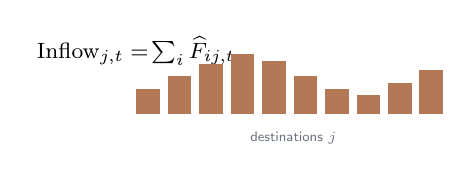
\begin{tikzpicture}[baseline=0]
        \node[font=\sffamily\footnotesize] at (0, 0) {$\mathrm{Inflow}_{j,t} = \!\sum_i \widehat{F}_{ij,t}$};
        % small bar chart of inflow per j
        \begin{scope}[shift={(0, -8mm)}]
          \foreach \j/\h in {0/0.4, 1/0.6, 2/0.8, 3/0.95, 4/0.85, 5/0.6, 6/0.4, 7/0.3, 8/0.5, 9/0.7}{
            \fill[stageCBanner!70]
                  (\j*4mm, 0) rectangle (\j*4mm + 3mm, \h*8mm);
          }
          \node[font=\sffamily\tiny, text=cMuted] at (20mm, -3mm) {destinations $j$};
        \end{scope}
      \end{tikzpicture}
    \end{minipage}};

  % ── Panel C2: BPR multiplier ──
  \node[modC, anchor=north west] (bpr) at (80mm, 0)
    {\begin{minipage}{84mm}
      \centering\textbf{\textcolor{stageCBanner}{\textcircled{\scriptsize 7} BPR multiplier · car-only}}\\[2pt]
      \scriptsize\textcolor{cIO}{IN: $\mathrm{Inflow}, C_j$}\;\;\textcolor{cIO}{OUT: $t^{(\text{car}),\text{cong}}_{ij,t}$}\\[3pt]
      \begin{tikzpicture}[baseline=0]
        \node[font=\sffamily\footnotesize] at (0, 8mm)
              {$t^{\text{cong}}\!=\!t_0\!\left(1{+}0.15\!\left(\frac{V}{C}\right)^4\right)$, cap 2.5};
        \includegraphics[width=58mm]{../figures/arch/bpr_v2.png}
        \node[font=\sffamily\tiny, text=cMuted] at (0, -16mm)
              {transit / walk $t$ unchanged};
      \end{tikzpicture}
    \end{minipage}};

  % ── Panel C3: MSA fixed-point loop ──
  \node[modC, anchor=north west] (msa) at (172mm, 0)
    {\begin{minipage}{128mm}
      \centering\textbf{\textcolor{stageCBanner}{\textcircled{\scriptsize 8} MSA fixed-point loop $\circlearrowleft$}}\\[2pt]
      \scriptsize\textcolor{cIO}{IN: $t^{(\text{car}),\text{cong}}$ updated}\;\;\textcolor{cIO}{OUT: equilibrium $\widehat{F}^{*}, t_{\text{eq}}$}\\[3pt]
      \begin{tikzpicture}[baseline=0]
        \node[font=\sffamily\scriptsize, anchor=west] at (0, 6mm)
              {$F^{(k+1)}\!=\!\left(1{-}\tfrac{1}{k}\right)F^{(k)} + \tfrac{1}{k}\,\mathrm{choice}\!\left(t^{(k)}\right)$};
        % Iteration sketch
        \foreach \k/\xoff in {1/0, 2/16, 3/32, 4/48, 5/64}{
          \node[draw=stageCBanner, fill=white, rounded corners=2pt, line width=0.4pt,
                 minimum width=12mm, minimum height=8mm,
                 font=\sffamily\tiny, text=stageCBanner]
                (it\k) at (\xoff mm, -8mm) {iter $k\!=\!\k$};
        }
        \foreach \k in {1,2,3,4} {
          \pgfmathtruncatemacro{\next}{\k+1}
          \draw[->, line width=0.5pt, draw=stageCBanner] (it\k.east) -- (it\next.west);
        }
        \node[font=\sffamily\tiny, text=cParBeta] at (38mm, -16mm)
              {converge: rel-gap\,$<\!0.5\%$};
        \node[font=\sffamily\tiny, text=cParBeta] at (38mm, -19mm)
              {Sc.\,A: 30 iter / Sc.\,B: 8 iter};
        % Loop arrow back to ⑤ (above)
        \draw[arrBPR] (38mm, 4mm) .. controls (38mm, 18mm) and (-100mm, 18mm) ..
              node[arrlbl, fill=white, font=\sffamily\scriptsize\itshape, text=cBPR]
                  {feedback: $t^{(\text{car})}\!\to\!\circlearrowleft$ choice}
              (-100mm, 12mm);
      \end{tikzpicture}
    \end{minipage}};

  % inner arrows
  \draw[arrInner] (inflow.east) -- node[arrlbl, above]{$\mathrm{Inflow}_j$} (bpr.west);
  \draw[arrInner] (bpr.east) -- node[arrlbl, above]{$t^{\text{cong}}$} (msa.west);

\end{scope}

\begin{pgfonlayer}{background}
  \node[rowframe=stageCBg, fit=(row3)] (frameRow3) {};
\end{pgfonlayer}
\node[rowbanner=stageCBanner, anchor=north west]
  at ($(frameRow3.north west)+(8pt, 0pt)$)
  {\textsc{Stage C · BPR closure + MSA fixed point}\;\,\textmd{\itshape — congestion feedback iterates choice $\circlearrowleft$ until equilibrium}};

% ════════════════════════════════════════════════════════════════════════
%  ROW 4 · OUTPUTS · WELFARE ASSESSMENT
% ════════════════════════════════════════════════════════════════════════

\begin{scope}[local bounding box=row4, shift={(0, -226mm)}]

  % ── Panel D1: Equilibrium F̂*, t_eq summary numbers ──
  \node[modD, anchor=north west] (eq) at (0, 0)
    {\begin{minipage}{84mm}
      \centering\textbf{\textcolor{stageDBanner}{\textcircled{\scriptsize 9} Equilibrium $\widehat{F}^{*}, t_{\text{eq}}$}}\\[2pt]
      \scriptsize\textcolor{cIO}{from MSA convergence}\\[3pt]
      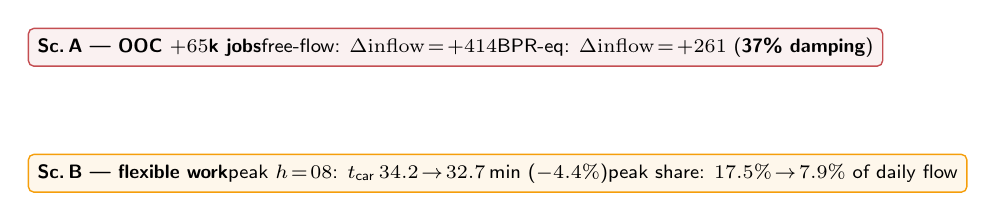
\begin{tikzpicture}[baseline=0]
        \node[draw=cParBeta, fill=cParBeta!8, rounded corners=2pt, line width=0.5pt,
               minimum width=72mm, font=\sffamily\scriptsize, anchor=north west]
              (sca_box) at (0, 0)
             {\textbf{Sc.\,A — OOC $+65$k jobs}\\
              free-flow: $\Delta\mathrm{inflow}\!=\!+414$\\
              BPR-eq: $\Delta\mathrm{inflow}\!=\!+261$ (\textbf{37\% damping})};
        \node[draw=cParGamma, fill=cParGamma!8, rounded corners=2pt, line width=0.5pt,
               minimum width=72mm, font=\sffamily\scriptsize,
               anchor=north west] (scb_box) at (0, -16mm)
             {\textbf{Sc.\,B — flexible work}\\
              peak $h\!=\!08$: $t_{\text{car}}\,34.2\!\to\!32.7\,$min ($-4.4\%$)\\
              peak share: $17.5\%\!\to\!7.9\%$ of daily flow};
      \end{tikzpicture}
    \end{minipage}};

  % ── Panel D2: Hansen accessibility heatmap (real London) ──
  \node[modD, anchor=north west] (access) at (92mm, 0)
    {\begin{minipage}{72mm}
      \centering\textbf{\textcolor{stageDBanner}{\textcircled{\scriptsize 10} Hansen accessibility $A_i$}}\\[2pt]
      \scriptsize $A_i\!=\!\sum_j E_j\,e^{\beta_{\text{car}} t_{ij,t}^{(\text{car}),\text{eq}}}$\\[3pt]
      \includegraphics[width=64mm]{../figures/arch/grid_accessibility_small.png}\\
      \scriptsize CBD-concentrated · max\,/\,p10 $\approx 25\!\times$
    \end{minipage}};

  % ── Panel D3: Welfare deltas (Gini / Palma) ──
  \node[modD, anchor=north west] (welfare) at (172mm, 0)
    {\begin{minipage}{128mm}
      \centering\textbf{\textcolor{stageDBanner}{\textcircled{\scriptsize 11} Welfare $\Delta$ — $\Delta$Gini, $\Delta$Palma}}\\[2pt]
      \scriptsize population-weighted inequality on $A_i$\\[3pt]
      \includegraphics[width=80mm]{../figures/arch/inequality_bars.png}\\
      \scriptsize \textbf{\textcolor{cParBeta}{Sc.\,A regressive}} ($\Delta$Gini\,${+}1.3\%$) \,vs\,
      \textbf{\textcolor{cAgentWalk}{Sc.\,B progressive}} ($\Delta$Gini\,${<}0$)\\[2pt]
      \scriptsize\textit{Same trained $\Theta$, opposite distributional verdicts — central policy finding}
    \end{minipage}};

  % inner arrows (data flow within outputs row)
  \draw[arrInner] (eq.east) -- (access.west);
  \draw[arrInner] (access.east) -- (welfare.west);

\end{scope}

\begin{pgfonlayer}{background}
  \node[rowframe=stageDBg, fit=(row4)] (frameRow4) {};
\end{pgfonlayer}
\node[rowbanner=stageDBanner, anchor=north west]
  at ($(frameRow4.north west)+(8pt, 0pt)$)
  {\textsc{Stage D · Outputs — counterfactual welfare assessment}\;\,\textmd{\itshape — equilibrium $\to$ accessibility $\to$ inequality}};

% ════════════════════════════════════════════════════════════════════════
%  MAIN VERTICAL FLOW ARROWS BETWEEN ROWS
% ════════════════════════════════════════════════════════════════════════

\draw[arrFwd] ($(frameRow1.south)+(0, 0)$) --
              node[arrlbl, fill=white, font=\sffamily\small\bfseries]
                  {$X^{\,\prime}+\Theta\!\bigstar$ frozen}
              ($(frameRow2.north)+(0, 0)$);
\draw[arrFwd] ($(frameRow2.south)+(0, 0)$) --
              node[arrlbl, fill=white, font=\sffamily\small\bfseries]{$\widehat{F}_{ij,t}$}
              ($(frameRow3.north)+(0, 0)$);
\draw[arrFwd] ($(frameRow3.south)+(0, 0)$) --
              node[arrlbl, fill=white, font=\sffamily\small\bfseries]{$\widehat{F}^{*}, t_{\text{eq}}$}
              ($(frameRow4.north)+(0, 0)$);

% ════════════════════════════════════════════════════════════════════════
%  Title and footer
% ════════════════════════════════════════════════════════════════════════

\node[font=\sffamily\bfseries\Large, anchor=south west, text=cText]
  at ($(frameRow1.north west)+(0, 8mm)$)
  {Figure 2 — ABM Forward Simulation Pipeline};
\node[font=\sffamily\itshape\large, anchor=south west, text=cMuted]
  at ($(frameRow1.north west)+(0, 4mm)$)
  {counterfactual deployment with frozen trained $\Theta$ + destination-side BPR closure};

\node[font=\sffamily\scriptsize\itshape, text=cMuted, anchor=north west,
       text width=300mm]
  at ($(frameRow4.south west)+(0, -6pt)$)
  {Stage A receives the 5 trained parameter types from Figure~1.\;
   Stage B re-encodes $X^{\,\prime}$ with frozen weights, samples $N$ heterogeneous agents from $(\pi_m, \pi_k)$, and dispatches each agent's individual Gumbel-max choice using their personal $(\beta_{t,m_n}, \kappa_{k_n}, \delta_{k_n})$.\;
   Stage C closes the destination-side congestion feedback loop until MSA convergence.\;
   Stage D reports equilibrium flow, Hansen accessibility, and population-weighted inequality measures.};

\end{tikzpicture}

\end{document}
